%%%%%%%%%%%%%%%%%%%%%%%%%%%%%%%%%%%%%%%%%%%%%%%%%%%%%%%%%%%%%%%%%%
%%%%%%%%%%%%%%%%%%%%%%%%%%% ANNEXES	 %%%%%%%%%%%%%%%%%%%%%%%%%%%%%
%%%%%%%%%%%%%%%%%%%%%%%%%%%%%%%%%%%%%%%%%%%%%%%%%%%%%%%%%%%%%%%%%%

\appendix
\chapter{Lien vers tout le code source de la chaîne de traitement \ktb{}}
L'intégralité du code produit pour le projet \ktb{}, depuis la création des documents \tei{} jusqu'à l'application Web, sont disponibles sur la plateforme d'hébergement de code GitHub.
\begin{itemize}
	\item \href{https://github.com/katabase}{Plateforme du projet}
	\item \href{https://github.com/katabase/1_OutputData}{Première étape: normalisation des documents \tei{}}
	\item \href{https://github.com/katabase/2_CleanedData}{Deuxième étape: extraction de données et normalisation}
	\item \href{https://github.com/katabase/3_WikidataEnrichment}{Troisième étape: enrichissement de données à l'aide de \wkd{}}
	\item \href{https://github.com/katabase/4_TaggedData}{Quatrième étape: création de jeux de données \json{} pour le site web}
	\item \href{https://github.com/katabase/Application}{Application web \ktb{}}
\end{itemize}

L'intégralité du code source est disponible sous licence libre (\href{https://www.gnu.org/licenses/gpl-3.0.html}{GNU GPL v3.0}, \href{https://mit-license.org/}{MIT} ou \href{https://creativecommons.org/}{Creative Commons}). Le site web peut également être consulté en ligne à \href{https://katabase.huma-num.fr/}{cette adresse}.


\chapter{Graphiques}
\begin{figure}
	\centering
	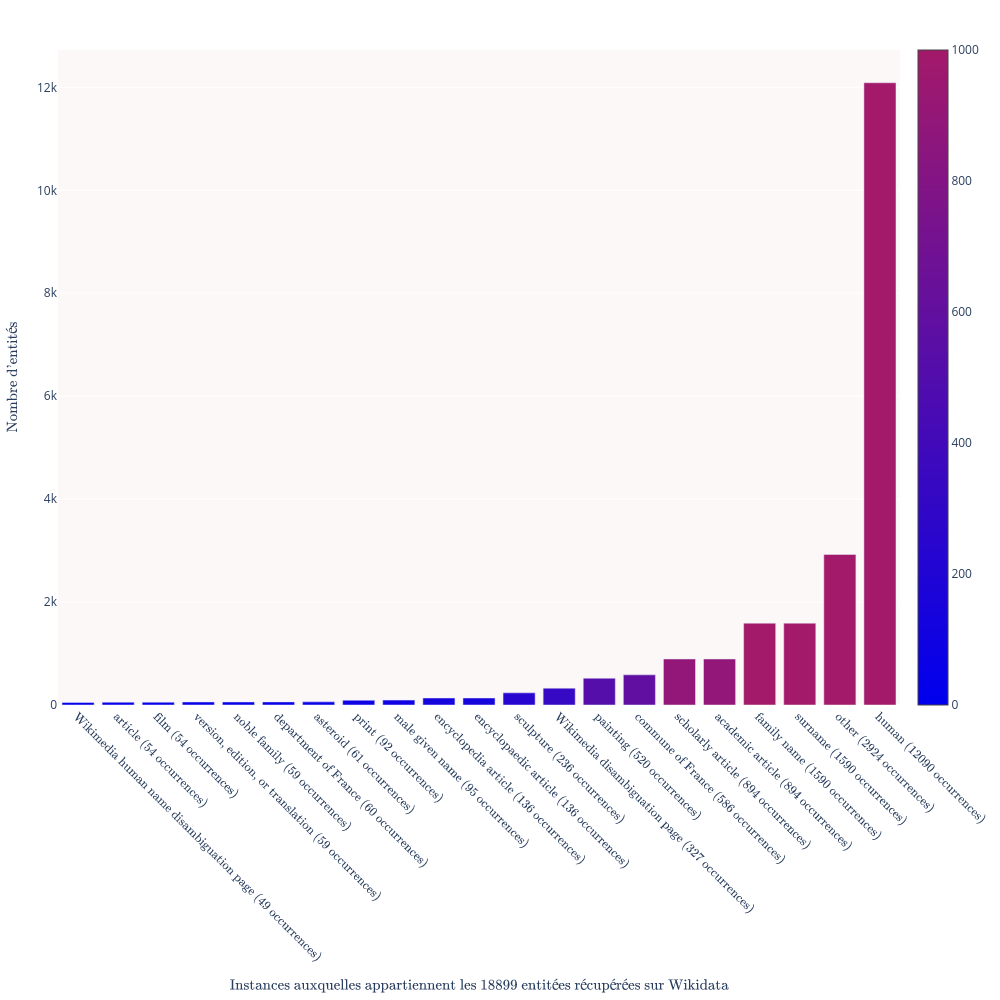
\includegraphics[width=\linewidth]{annexes/fig_wikidata_instances.png}
	\caption \\Occurrences des différentes catégories auxquelles appartiennent les entités \wkd{} liées avec les entrées de catalogues
	\label{appendix:wikidata_instances}
\end{figure}

\begin{figure}
	\centering
	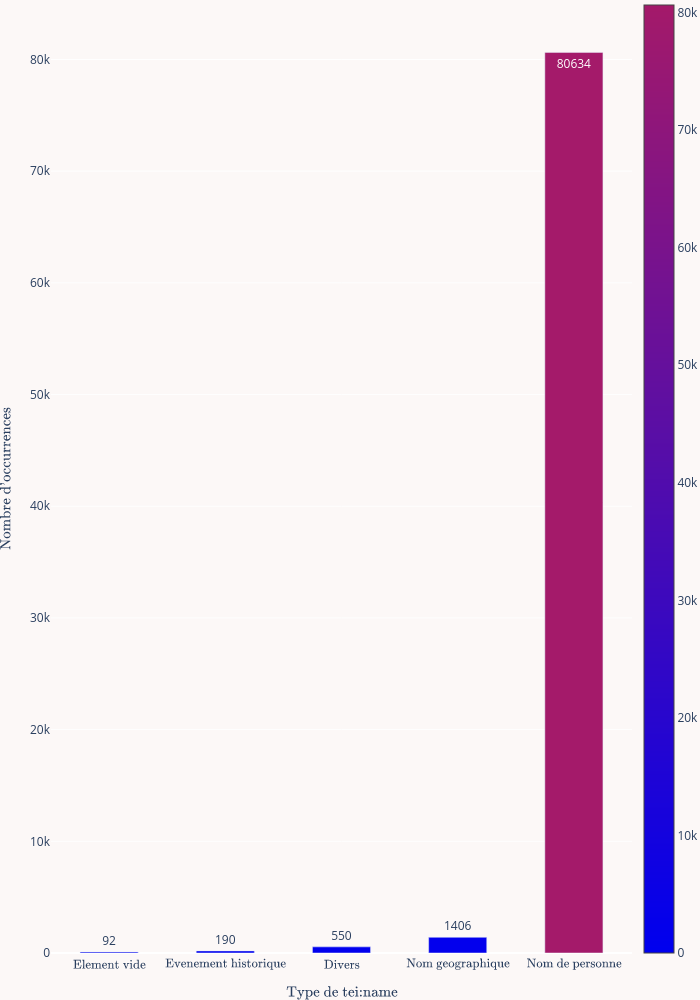
\includegraphics[width=\linewidth]{annexes/fig_teinametypes.png}
	\caption{Répartition des différents types de \tname{}}
	\label{appendix:tnametypes}
\end{figure}

\chapter{Code source et données encodées}
\begin{listing}[p]
	\begin{minted}{python}
functions = {
	"général": "general",
	"maréchal": "marshal",
	"lieutenant": "military",
	"officier": "military",
	"colonel": "military",
	"lieutenant-colonel": "military",
	"commandant": "military",
	"capitaine": "military",  # "less important" military positions
	"roi": "king",
	"empereur": "emperor",
	"president": "president",
	"homme politique": "politician",
	"président de l'assemblée": "politician",
	"orateur": "politician",
	"député": "politician",
	"secrétaire d'état": "politician",
	"sénateur": "politician",
	"écrivain": "writer",
	"auteur": "writer",
	"romancier": "writer",
	"acteur": "actor",
	"actrice": "actress",
	"cantatrice": "singer",
	"chanteur": "singer",
	"chanteuse": "singer",
	"peintre": "painter",
	"sculpteur": "sculptor",
	"statutaire": "sculptor",
	"compositeur": "composer",
	"musicien": "musician",
	"musicienne": "musician",
	"tragédien": "actor",
	"chansonnier": "chansonnier",
	"achitecte": "architect",
	"journaliste": "journalist",
	"inventeur": "inventor",
	"chimiste": "chemist",
	"connétable": "constable",
	"archevêque": "archbishop",
	"évêque": "bishop",
	"docteur": "physicist",
	"médecin": "physicist"
}		
	\end{minted}
	\caption{Table de conversion associant un métier à son équivalent normalisé}
	\label{appendix:convfunction}
\end{listing}


\begin{listing}[p]
	\begin{minted}{python}
dpts = [
	"ain",
	"aisne",
	"allier",
	"basses-alpes",
	"hautes-alpes",
	"alpes-maritimes",
	"annepins",
	"provence",
	"ardèche",
	"ardennes",
	"arriège",
	"arno",
	"aube",
	"aude",
	"aveyron",
	"bouches-de-l'elbe",
	"bouches-de-l'escaut",
	"bouches-de-l'yssel",
	"bpuches-de-la-meuse",
	"bouches-du-rhin",
	"bouches-du-rhône",
	"bouches-du-weser",
	"calvados",
	"cantal",
	"charente",
	"charente-inférieure",
	"cher",
	"corrèze",
	"corse",
	"côte-d'or",
	"côtes-du-nord",
	"creuse",
	"deux-nèthes",
	"deux-sèvres",
	"doire",
	"dordogne",
	"doubs",
	"drôme",
	"dyle",
	"ems-occidental",
	"ems-oriental",
	"ems-supérieur",
	"escaut",
	"eure",
	"eure-et-loir",
	"finistère",
	"forêts",
	"gard",
	"haute-garonne",
	"gers",
	"gironde",
	"hérault",
	"ille-et-villaine",
	"indre",
	"indre-et-loire",
	"isère",
	"jemappes",
	"jura",
	"landes",
	"léman",
	"loire",
	"loir-et-cher",
	"haute-loire",
	"loire-inférieure",
	"loiret",
	"lot",
	"lot-et-garonne",
	"lozère",
	"lys",
	"maine-et-loire",
	"manche",
	"marengo",
	"marne",
	"haute-marne",
	"méditerrannée",
	"mayenne",
	"meurthe",
	"meuse",
	"meuse-inférieure",
	"mont-blanc",
	"mont-tonnerre",
	"montenotte",
	"morbihan",
	"meuse",
	"moselle",
	"nièvre",
	"nord",
	"oise",
	"ombrone",
	"orne",
	"ourte",
	"paris",
	"pas-de-calais",
	"pô",
	"puy-de-dôme",
	"hautes-pyrénées",
	"basses-pyrénées",
	"pyrénées-orientales",
	"haut-rhin",
	"bas-rhin",
	"rhin-et-moselle",
	"rhône",
	"rhône-et-loire",
	"roer",
	"rome",
	"haute-saône",
	"saône-et-loire",
	"sambre-et-meuse",
	"sarre",
	"sarthe",
	"seine",
	"seine-et-marne",
	"seine-et-oise",
	"seine-inférieure",
	"sézia",
	"simplon",
	"deux-sèvres",
	"somme",
	"stura",
	"tarn",
	"tarn-et-garonne",
	"taro",
	"trasimène",
	"var",
	"vaucluse",
	"vendée",
	"vienne",
	"haute-vienne",
	"vosges",
	"yonne",
	"yssel-supérieur",
"zuyderzée"
]		
	\end{minted}
	\caption{Liste de départements du XIXe~s. pour détecter des informations géographiques}
	\label{appendix:convdpt}
\end{listing}

\begin{listing}[p]
	\begin{minted}{python}
countries = {
	"états-unis d'amérique": "united states of america",
	"etats-unis d'amérique": "united states of america",
	"états unis d'amérique": "united states of america",
	"etats unis d'amerique": "united states of america",
	"états-unis": "united states of america",
	"etats-unis": "united states of america",
	"etats unis": "united states of america",
	"états unis": "united states of america",
	"italie": "italy",
	"grèce": "greece",
	"canada": "canada",
	"chine": "china",
	"haïti": "haiti",
	"tobago": "tobago",
	"brésil": "brasil",
	"burkina-faso": "burkina-faso",
	"cameroun": "cameroun",
	"tchad": "tchad",
	"congo": "congo",
	"gabon": "gabon",
	"guinée": "guinea",
	"côte d'ivoire": "ivory coast",
	"mali": "mali",
	"mauritanie": "mauritania",
	"niger": "niger",
	"sénégal": "senegal",
	"madagascar": "madagascar",
	"seychelles": "seychelles",
	"tanzanie": "tanzania",
	"zanzibar": "zanzibar",
	"liban": "lebanon",
	"syrie": "syria",
	"inde": "india",
	"laos": "laos",
	"viet-nâm": "vietnam"
}	
	\end{minted}
	\caption{Table de conversion pour les pays}
	\label{appendix:convcountry}
\end{listing}

\begin{listing}[p]
	\begin{minted}{python}
colonies = [
	"québec",
	"ontario",
	"saint-pierre-et-miquelon",
	"mississippi",
	"missouri",
	"louisiane",
	"anguilla",
	"antigua",
	"dominique",
	"saint-domingue",
	"guadeloupe",
	"monsterrat",
	"saint-martin",
	"saint-barthélémy",
	"sainte-lucy",
	"saint-vincent-et-les-grenadines",
	"saint-eustache",
	"saint-christophe",
	"martinique"
	"guyane française",
	"guyane",
	"maroc",  # unfortunately the morocco referred to in XIXth century france is a french protectorate
	"algérie",  # same
	"algérie française",  # same
	"tunisie",  # same
	"fezzan",
	"dahomey",
	"haute-volta",
	"oubangui-chari",
	"congo français",
	"moyen-congo",
	"guinée française",
	"soudan français",
	"gorée",
	"tigi",
	"djibouti",
	"cheikh saïd",
	"comores",
	"fort-dauphin",
	"îles maurice",
	"mayotte",
	"la réunion",
	"îles éparses",
	"île amsterdam",
	"île saint-paul",
	"archipel crozet",
	"îles kerguelen",
	"castellorizo",
	"grand-liban",
	"sandjak d'alexandrette",
	"indes françaises",
	"pondichéry",
	"karikal",
	"yanaon",
	"mahé",
	"chanderngor",
	"tonkin",
	"annam",
	"cochinchine",
	"guangzhou wan",
	"shanghai",
	"guangzhou",
	"tianjin",
	"hankou",
	"clipperton",
	"nouvelle-calédonie",
	"polynésie française",
	"vanuatu",
	"nouvelles-hébrides",
	"wallis et futuna"
]
	\end{minted}
	\caption{Liste d'anciennes colonies françaises pour la détection de motifs}
	\label{appendix:convcolonie}
\end{listing}

\begin{listing}[p]
	\begin{minted}{python}
provinces = [
	"armagnac",
	"île-de-france",
	"berry",
	"orléanais",
	"normandie",
	"languedoc",
	"lyonnais",
	"dauphiné",
	"champagne",
	"aunis",
	"saintonge",
	"poitou",
	"guyenne et gascogne",
	"bourgogne",
	"picardie",
	"anjou",
	"provence",
	"angoumois",
	"bourbonnais",
	"marche",
	"bretagne",
	"maine",
	"touraine",
	"limousin",
	"comté de foix",
	"auvergne",
	"béarn",
	"alsace",
	"artois",
	"roussillon",
	"flandre française et hainaut français",
	"franche-comté",
	"lorraine et trois-évêchés",
	"corse",
	"nivernais",
]
	\end{minted}
	\caption{Liste d'anciennes provinces françaises pour la détection de motifs}
	\label{appendix:convprov}
\end{listing}

\begin{listing}[p]
	\begin{minted}{python}
events = {
	"défense nationale": "government of national defense",
	"defense nationale": "government of national defense",
	"révolution française": "french revolution",
	"revolution francaise": "french revolution",
	"guerre de trente ans": "thirty years' war 1618 1648",
	"guerre de cent ans": "hundred years' war 1337 1453",
	"guerre de sept ans": "seven years war 1756 1763",
	"guerre": "war",
	"insurrection": "war",
	"siège de mayence": "siege of mainz",
	"siège": "siege",
	"commune": "commune",
	"défense": "battle",
	"révolution": "revolution"
}
	\end{minted}
	\caption{Table de conversion pour les évènements historiques}
	\label{appendix:convevt}
\end{listing}

\begin{listing}[p]
	\begin{minted}{python}
status = {
	"empereur": "",
	"impératrice": "",
	"géneral": "general",
	"reine": "queen",
	"roi": "king",
	"princesse": "princess",
	"prince": "prince",
	"archiduchesse": "",
	"archiduc": "",
	"duchesse": "duchess",
	"duc": "duke",
	"famille": "family",
	"seigneur": "",
	"vicomtesse": "",
	"victesse": "",
	"vicomte": "",
	"victe": "",
	"comtesse palatine": "countess palatine",
	"comtesse": "",
	"ctesse": "",
	"comte": "",
	"cte": "",
	"cardinal": "",
	"pape": "pope",
	"lord": "",
	"chevalier": "",
	"marquise": "",
	"marquis": "",
	"sire": "",
	"baronnesse": "",
	"baronne": "",
	"baron": "",
	"abbé": "",
	"madame": "",
	"mme": "",
	"monsieur": "",
	"mr": "",
	"docteur": "",
	"maréchale": "",
	"maréchal": "",
	"mademoiselle": "",
	"melle": "",
	"mlle": "",
	"sir": ""
}
	\end{minted}
	\caption{Liste de colonies pour la détection de motifs}
	\label{appendix:convstatus}
\end{listing}

\begin{listing}[p]
	\begin{minted}{python}
comp_names = {
	"arm ch": "armand-charles",
	"ch m": "charles-marie",
	"ch l f": "charles-louis-françois",
	"f m": "francois-marie",
	"fr emm.": "françois-emmanuel",
	"j ant": "jean-antoine",
	"j f": "jean-francois",
	"j m": "jean-marie",
	"j j": "jean-jacques",
	"j l": "jean-louis",
	"j b": "jean-baptiste",
	"j p": "jean-pierre",
	"j pierre": "jean-pierre",
	"l f": "louis-françois",
	"m f": "marius-felix",
	"franc rené": "francois-rené",
	"m madeleine": "marie-madeleine",
	"ph h": "philippe henri",
	"p aug": "pierre auguste",
	"p alex": "pierre alexandre",
	"p j": "pierre-jean",
	"j sylvain": "jean-sylvain",
	"l ph": "louis-philippe",
	"edm ch": "edmond-charles",
	"ch marie": "charles-marie"
}
	\end{minted}
	\caption{Table de conversion permettant de remplacer un nom abrégé composé par sa version complète}
	\label{appendix:namecomp}
\end{listing}

\begin{listing}[p]
	\begin{minted}{python}
names = {
	"ad": "adam",
	"alex": "alexandre",
	"alph": "alphonse",
	"ant": "antoine",
	"arm": "armand",
	"aug": "auguste",
	"ch": "charles",
	"cl": "claude",
	"dom": "dominique",
	"emm": "emmanuel",
	"ed": "edouard",
	"et": "etienne",
	"ét": "etienne",
	"ferd": "ferdinand",
	"fred": "frederic",
	"fr": "françois",
	"franc": "françois",
	"franç": "françois",
	"fréd": "frédéric",
	"g": "guillaume",
	"guill": "guillaume",
	"gab": "gabriel",
	"jh": "joseph",
	"jacq": "jacques",
	"jos": "joseph",
	"math": "matthieu",
	"nic": "nicolas",
	"ph": "philippe",
	"v": "victor",
	"vr": "victor",
}
	\end{minted}
	\caption{Table de conversion permettant de remplacer un nom abrégé non composé par sa version complète}
	\label{appendix:namesimp}
\end{listing}

\begin{listing}[p]
	\begin{minted}[breakanywhere]{python}
def rgx_abvcomp(nstr):
	"""
	try to extract an abbreviated composed first name. if there is no match, return None
	pattern
	-------
	the patterns in the example below are simplified to keep things readable
	- two strings separated by a "-" or "\s"
	- the first or second string can be a full name ([A-Z][a-z]+)
	or an abbreviation ([A-Z][a-z]*\.)
	- if the strings are separated by "\s", they must be finished by "\."
	(to be sure that we don't capture full names, i.e: "J. Ch."  can be captured,
	but not "Jean Charles")
	- complex names with 3 or more words must have "-" and at least one "\."
	- (\s|$) and (^|\s) are safeguards to avoid matching the end or beginning of another word
	examples
	--------
	matched : M.-Madeleine Pioche de la Vergne  # matched string : M.-Madeleine
	matched : C.-A. de Ferriol  # matched string : C.-A.
	matched : J. F.  # matched string : J. F.
	matched : Jean F.  # matched string : Jean F.
	matched : Jean-F.  # matched string : Jean-F.
	matched : A M  # matched string : A M
	matched : C.-Edm.-G.  # matched string : C.-Edm.-G.
	matched : Charles-Edm.-G.  # matched string : Charles-Edm.-G.
	not matched : Anne M
	not matched : Claude Henri blabla
	not matched : Claude Henri
	:param nstr: the name string used as input
	:return: the matched string if there is a match ; None if there is no match
	"""
	mo = re.search(r"(^|,|\s)[A-ZÀÂÄÈÉÊËÏÔŒÙÛÜŸ][a-zàáâäéèêëíìîïòóôöúùûüøœæç]*"
			+ "\.?-[A-ZÀÂÄÈÉÊËÏÔŒÙÛÜŸ][a-zàáâäéèêëíìîïòóôöúùûüøœæç]*\.(\s|,|$)", nstr) \
		 or re.search(r"(^|,|\s)[A-ZÀÂÄÈÉÊËÏÔŒÙÛÜŸ][a-zàáâäéèêëíìîïòóôöúùûüøœæç]*\."
			+ "-[A-ZÀÂÄÈÉÊËÏÔŒÙÛÜŸ][a-zàáâäéèêëíìîïòóôöúùûüøœæç]*\.?(\s|,|$)", nstr) \
		 or re.search(r"(^|,|\s)[A-ZÀÂÄÈÉÊËÏÔŒÙÛÜŸ]\.?\s"
			+ "[A-ZÀÂÄÈÉÊËÏÔŒÙÛÜŸ][a-zàáâäéèêëíìîïòóôöúùûüøœæç]*\.(\s|,|$)", nstr) \
		 or re.search(r"(^|,|\s)[A-ZÀÂÄÈÉÊËÏÔŒÙÛÜŸ][a-zàáâäéèêëíìîïòóôöúùûüøœæç]*\.?"
		    + "\s[A-ZÀÂÄÈÉÊËÏÔŒÙÛÜŸ]\.(\s|,|$)", nstr) \
		 or re.search(r"(^|,|\s)[A-ZÀÂÄÈÉÊËÏÔŒÙÛÜŸ]\.?\s[A-ZÀÂÄÈÉÊËÏÔŒÙÛÜŸ]\.?(\s|,|$)", nstr) \
		 or re.search(r"([A-ZÀÂÄÈÉÊËÏÔŒÙÛÜŸ]\.){2,}", nstr) \
		 or re.search(r"(^|,|\s)([A-ZÀÂÄÈÉÊËÏÔŒÙÛÜŸ][a-zàáâäéèêëíìîïòóôöúùûüøœæç]*\.?-)+"
			+ "([A-ZÀÂÄÈÉÊËÏÔŒÙÛÜŸ][a-zàáâäéèêëíìîïòóôöúùûüøœæç]*\.)(\s|,|$)", nstr) \
		 or re.search(r"(^|,|\s)([A-ZÀÂÄÈÉÊËÏÔŒÙÛÜŸ][a-zàáâäéèêëíìîïòóôöúùûüøœæç]*\.-)+"
		  	+ "([A-ZÀÂÄÈÉÊËÏÔŒÙÛÜŸ][a-zàáâäéèêëíìîïòóôöúùûüøœæç]*\.?)(\s|,|$)", nstr)
	if mo is not None:
		return mo[0]
	else:
		return None
	\end{minted}
	\caption{Fonction permettant d'identifier et d'extraire un nom abrégé composé}
	\label{appendix:rgxabvcomp}
\end{listing}

\begin{listing}[p]
	\begin{minted}[breakanywhere]{python}
def rgx_abvsimp(nstr):
	"""
	try to extract a "simple" (not composed) abbreviated first name. if there is no match, return None
	pattern
	-------
	a capital letter (possibly followed by a certain number of lowercase letters)
	ended with a dot. (\s|$) and (^|\s) are safeguards to avoid matching the beginning
	end of another word.
	*warning* : it can also capture parts of composed abbreviated names => must be used
	in an if-elif after trying to match a composed abbreviated name
	examples
	--------
	matched : bonjour Ad.  # matched string : Ad.
	matched : J. baronne  # matched string : J.
	matched : J. F.  # matched string : J.
	matched : Jean F.  # matched string : F.
	not matched : A.-M.
	not matched : Anne M
	not matched : Hector
	:param nstr: the name string used as input
	:return:
	"""
	mo = re.search(r"(^|\s)[A-ZÀÂÄÈÉÊËÏÔŒÙÛÜŸ][a-zàáâäéèêëíìîïòóôöúùûüøœæç]*\.(\s|$|,)", nstr)
	if mo is not None:
		return mo[0]
	else:
		return None
	\end{minted}
	\caption{Fonction permettant de repérer et d'extraire un nom abrégé simple}
	\label{appendix:rgxabvsimp}
\end{listing}

\begin{listing}[p]
	\begin{minted}[breakanywhere]{python}
def rgx_complnm(nstr):
	"""
	try to extract a complete name from a string. if there is no match, return None
	pattern
	-------
	- an uppercase letter followed by several lowercase letters ;
	- this pattern can be repeated several times, separated by a space or "-"
	- (\s|$) and (^|\s) are safeguards to avoid matching the beginning or end of another word.
	:param nstr: the string from which a name should be extracted
	:return:
	"""
	mo = re.search(r"(^|\s)[A-ZÀÂÄÈÉÊËÏÔŒÙÛÜŸ][a-zàáâäéèêëíìîïòóôöúùûüøœæç]+"
		+ "((\s|-)[A-ZÀÂÄÈÉÊËÏÔŒÙÛÜŸ][a-zàáâäéèêëíìîïòóôöúùûüøœæç]+)*($|\s|,)", nstr)
	if mo is not None:
		return mo[0]
	else:
		return None
	\end{minted}
	\caption{Fonction permettant d'identifier et d'extraire un nom complet non abrégé}
	\label{appendix:rgxfull}
\end{listing}